\documentclass{article}
\usepackage{amsmath}

\usepackage{graphicx}

\usepackage{listings}
\usepackage{color}
\definecolor{dkgreen}{rgb}{0,0.6,0}
\definecolor{gray}{rgb}{0.5,0.5,0.5}
\definecolor{mauve}{rgb}{0.58,0,0.82}
\lstset{frame=tb,
  language=R,
  aboveskip=3mm,
  belowskip=3mm,
  showstringspaces=false,
  columns=flexible,
  basicstyle={\small\ttfamily},
  numbers=none,
  numberstyle=\tiny\color{gray},
  keywordstyle=\color{blue},
  commentstyle=\color{dkgreen},
  stringstyle=\color{mauve},
  breaklines=false,
  breakatwhitespace=true,
  tabsize=3
}

\title{SDS385 Fall '16: Statistical Models For Big Data\\Exercises 03 - Line search}
\author{Matteo Vestrucci}
\date{September 21st 2016}
\begin{document}
\maketitle
\bigskip\bigskip\bigskip

\subsubsection*{A)}

The Backtracking Line Search Algorithm offers a different paradigm to set the step size of our gradient descent, compared to the fixed step size and the decaying step size. The pseudo algorithm to decide the size step at iteration $k$ is the following:

\begin{itemize}
\item initialize $\alpha_{max}>0$, $\rho \in (0,1)$, $c_1 \in (0,1)$, $\alpha=\alpha_{max}$
\item until $l\left(\beta_k-\alpha\cdot\nabla l(\beta_k)\right) \enskip\leq\enskip l(\beta_k)-c_1\cdot\alpha\cdot\nabla l(\beta_k)^T\nabla l(\beta_k)$ repeat $\alpha=\rho\cdot\alpha$ 
\item return $\alpha$
\end{itemize}

We consider a maximum step size $\alpha_{max}$ and then start reducing it until it meets a certain condition, called Armijo Condition or First Wolfe Condition. The condition is such that we are guaranteed to have at least some improvement in the objective function -compared to the previous iteration- proportional to the step $\alpha$ and a constant $c_1$. The idea is that the furthest we want to move the bigger must be the gain, to fight over-sized steps. A Second Wolfe Condition has been proposed to deal with under-sized steps but it's not integrated in the Backtracking Line Search Algorithm. Notice that it's impossible to get stuck in an infinite loop because the smaller it becomes the step, the smaller it becomes the requirement. To be noted also that we are guaranteed some improvement, and that's not as saying that we are getting the best possible along that direction. The suggested values are $c_1=0.0001$ and $\rho=0.9$.

\subsubsection*{B)}

Running the code in appendix, we can observe how the gradient descent with fixed step compares versus the gradient descent with line search.

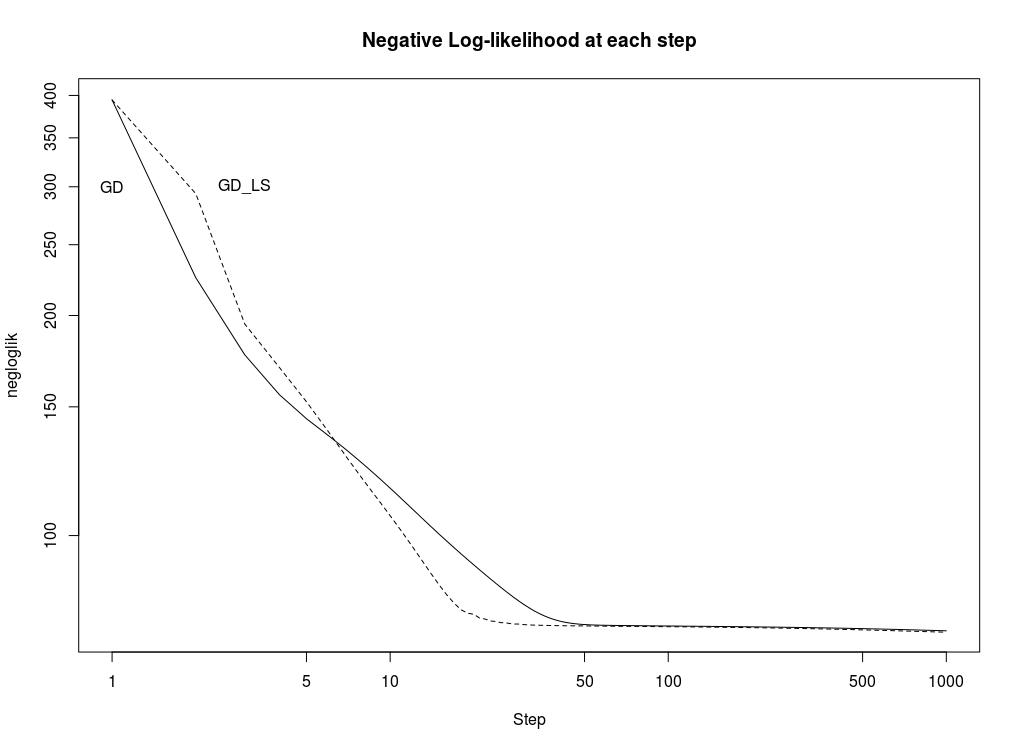
\includegraphics[width=\textwidth]{Rplot_line_search.png}

With the specific parameters presented in the code, it appears that in the first few iterations the fixed step size offers better improvements, but the line search quickly catches up and reaches pseudo convergence in half of the iterations required by the fixed step. It seems to be the case that the fixed step 0.2 is more suited at the beginning but then it tends to be a bit bigger than necessary later on. The line search starts at 0.6 but it's able to decrease that amount when the improvements don't satisfy anymore the minimum amount set by the condition and a smaller step offers instead better returns in proportion.\\

\begin{tabular}{llllllll}
&\multicolumn{7}{l}{Unit:seconds} \\
&      &min      &  lq     & mean     & median   &     uq   &    max   \\
&GD   &1.78  &1.78 & 1.79 & 1.78 & 1.79 & 1.88 \\
&GD\_ LS&10.57 &10.58& 10.70& 10.62& 10.88& 10.95\\
&\multicolumn{7}{l}{} 
\end{tabular}

It is a given that this comes with a price: instead of using always the same value we have to choose one at each iteration with a loop, and this costs us time. The benchmark shows us that line search is significantly slower in the case of gradient descent. It's not the loop itself the bottleneck but the fact that we are using the full negative loglikelihood to evaluate the condition of the loop, which entails going through all the dataset for each candidate $\alpha$. For this reason I set $\rho$ smaller than the suggested value in order to accept a candidate step in less tries. Line search seems very promising for Stochastic Gradient Descent, where we'll use a single observation to evaluate the negative loglikelihood.

\newpage

\subsubsection*{CODE)}

%[basicstyle=\tiny]
\begin{lstlisting}[basicstyle=\small]
library(Matrix)
library(microbenchmark)

negloglikelihood<-function(m,y,X,beta){
  total<-0
  N<-length(y)
  for(i in 1:N) total<-total+(m[i]-y[i])*t(X[i,])%*%beta+m[i]*log(1+exp(-t(X[i,])%*%beta))
  return(total)
}
gradient_negloglik<-function(m,y,X,beta){
  w<-1/(1+exp(-X%*%beta))
  S<-m*w-y
  grad<-t(X)%*%S
  return(grad)
}
gradient_descent<-function(m,y,X,beta0,stepsize,maxstepnumber,
							accuracy_obj_fun,accuracy_beta_val){
  negloglik<-numeric(maxstepnumber)
  negloglik[1]<-negloglikelihood(m,y,X,beta0)
  gradient<-gradient_negloglik(m,y,X,beta0)
  diff_beta_val<-accuracy_beta_val+1
  diff_obj_fun<-accuracy_obj_fun+1
  i<-1
  while(!(i==maxstepnumber)&&
  	    ((accuracy_beta_val<diff_beta_val)||(accuracy_obj_fun<diff_obj_fun))){
    i<-i+1
    beta1<-beta0-stepsize*gradient
    diff_beta_val<-sum(abs(beta0-beta1))
    beta0<-beta1
    negloglik[i]<-negloglikelihood(m,y,X,beta0)
    diff_obj_fun<-negloglik[i-1]-negloglik[i]
    gradient<-gradient_negloglik(m,y,X,beta0)}
  return(list(betahat=beta0,negloglik=negloglik,step=i))
}
line_search<-function(alpha,c1,rho,gradient,m,y,X,beta){
  while(negloglikelihood(m,y,X,(beta-alpha*gradient))>
        negloglikelihood(m,y,X,beta)+c1*alpha*crossprod(gradient))
    alpha<-alpha*rho
  return(alpha)
}
line_search_gd<-function(m,y,X,beta0,maxstepnumber,alpha,c1,rho,
						  accuracy_obj_fun,accuracy_beta_val){
  negloglik<-numeric(maxstepnumber)
  negloglik[1]<-negloglikelihood(m,y,X,beta0)
  gradient<-gradient_negloglik(m,y,X,beta0)
  diff_beta_val<-accuracy_beta_val+1
  diff_obj_fun<-accuracy_obj_fun+1
  i<-1
  while(!(i==maxstepnumber)&&
  	    ((accuracy_beta_val<diff_beta_val)||(accuracy_obj_fun<diff_obj_fun))){
    i<-i+1
    stepsize<-line_search(alpha,c1,rho,gradient,m,y,X,beta0)
    beta1<-beta0-stepsize*gradient
    diff_beta_val<-sum(abs(beta0-beta1))
    beta0<-beta1
    negloglik[i]<-negloglikelihood(m,y,X,beta0)
    diff_obj_fun<-negloglik[i-1]-negloglik[i]
    gradient<-gradient_negloglik(m,y,X,beta0)}
  return(list(betahat=beta0,negloglik=negloglik,step=i))
}

data_wdbc<-read.csv("./wdbc.csv", header=FALSE)
X<-as.matrix(cbind(rep(1,569),scale(data_wdbc[,3:12])))
y<-data_wdbc[,2]
y<-as.numeric(y=="M")
m<-rep(1,569)

beta0<-rep(0,11)
stepsize<-0.02
alpha<-0.06
c1<-0.0001
rho<-2/3
maxstepnumber<-1000
accuracy_obj_fun<-0.001
accuracy_beta_val<-0.001
result_grad_desc<-gradient_descent(m,y,X,beta0,stepsize,maxstepnumber,
                                   accuracy_obj_fun,accuracy_beta_val)
result_line_search<-line_search_gd(m,y,X,beta0,maxstepnumber,alpha,c1,rho,
                                   accuracy_obj_fun,accuracy_beta_val)
result_grad_desc$betahat
result_line_search$betahat

plot(result_grad_desc$negloglik[1:result_grad_desc$step],
     main = "Negative Log-likelihood at each step",
     xlab="Step",ylab="negloglik",type="l",log="xy")
points(result_line_search$negloglik[1:result_line_search$step],
       type="l",lty=2)
text(1, 300, "GD");text(3, 300, "GD_LS")

maxstepnumber<-100
microbenchmark(times=10,
result_grad_desc<-gradient_descent(m,y,X,beta0,stepsize,maxstepnumber,
                                   accuracy_obj_fun,accuracy_beta_val),
result_line_search<-line_search_gd(m,y,X,beta0,maxstepnumber,alpha,c1,rho,
                                   accuracy_obj_fun,accuracy_beta_val))
\end{lstlisting}

\end{document}